\begin{frame}{The Computational Graph}
    \framesubtitle{Visualizing Backpropagation}
    \begin{itemize}
        \item To manage the complexity of the chain rule in deep networks, we can represent the network as a \bhighlight{computational graph}.
        \item \textbf{Structure:} The graph consists of:
        \begin{itemize}
            \item \bhighlight{Nodes:} Represent operations (e.g., multiplication, addition, activation functions).
            \item \bhighlight{Edges:} Represent the flow of data (tensors) between nodes.
        \end{itemize}
    \end{itemize}
\end{frame}

\begin{frame}{The Computational Graph}
    \framesubtitle{Forward Pass}
    \begin{itemize}
        \item The \bhighlight{forward pass} involves evaluating the graph from the inputs to the final loss.
        \item Each node takes inputs and computes an output, which is then passed along to the next nodes.
    \end{itemize}
    \begin{figure}
        \centering
        % Source: MLP & Back-prop.pdf, Page: 40
        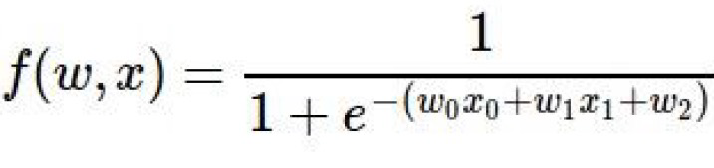
\includegraphics[width=0.9\linewidth]{images/computational_graph_sigmoid.png}
        \caption{A detailed computational graph for a single sigmoid neuron. The forward pass flows from left to right.}
    \end{figure}
\end{frame}

\begin{frame}{The Computational Graph}
    \framesubtitle{Backward Pass}
    \begin{itemize}
        \item \bhighlight{Backpropagation} is the process of applying the chain rule at each node to compute gradients, moving backward from the final output (the loss).
        \item Each node receives an "\bhighlight{upstream gradient}" (the gradient of the final loss with respect to the node's output).
        \item It then calculates its "\bhighlight{local gradient}" (the derivative of its output with respect to its inputs).
        \item The "\bhighlight{downstream gradient}" (the gradient to be passed to its inputs) is computed by multiplying the upstream gradient by the local gradient:
        \[
            \frac{\partial L}{\partial x} = \frac{\partial L}{\partial z} \frac{\partial z}{\partial x}
        \]
    \end{itemize}
\end{frame}

\begin{frame}{The Computational Graph}
    \framesubtitle{Example "Gates"}
    \begin{itemize}
        \item Different nodes (or "gates") distribute gradients differently:
    \end{itemize}
    \begin{figure}
        \centering
        % Source: MLP & Back-prop.pdf, Page: 38
        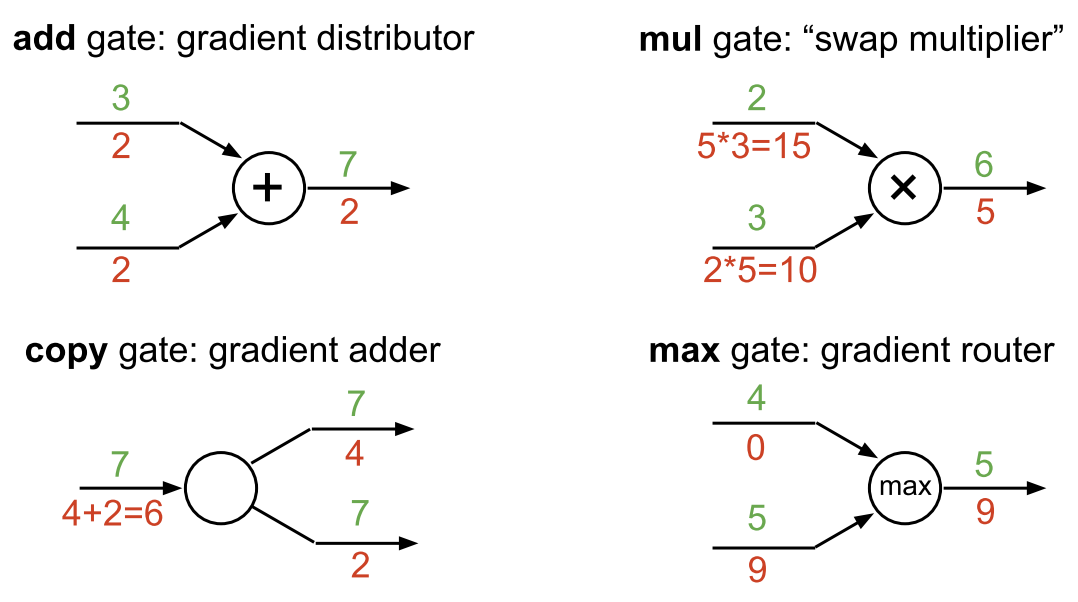
\includegraphics[width=\linewidth]{images/gradient_gates.png}
        \caption{Simple gates and their backpropagation behavior: Add gate distributes, Max gate routes, and Mul gate swaps and multiplies.}
    \end{figure}
\end{frame}